\renewcommand{\algorithmicrequire}{\textbf{Dados: }}
\renewcommand{\algorithmicensure}{\textbf{Resultado: }}

\section{Decomposição $k$-Core}


\subsection{Definição}
Sendo $G = (V,E)$ um grafo com $n = |V|$ vértices e $m = |E|$ arestas, $degree(u)$ o grau do vértice $u$, $G(C) = (C, E|C)$ um sub-grafo de G induzido pelo subconjunto de nós $C$ onde $E|C = \{(u,v)\subset E : u,v \subset C\} $ temos as seguintes definições relacionadas com a decomposição $k$-Core \cite{kCoreDef}:


	\begin{enumerate}
		\item Um sub-grafo $G(C)$ é uma $k$-core se e só se para todos os vértices pertencentes a $C$ o seu grau é maior ou igual a $k$ e $G(C)$é um grafo maximal.
		\item Um nó de $G$ diz-se ter \textit{coreness} se e só se este pertence à $k$-core mas não a $(k+1)-core$.
	\end{enumerate}


Assim, é possível conseguir-se as $k$-Cores de G removendo recursivamente todos os vértices cujo grau sejam menor que $k$.

Batagelj-Zaversnik apresenta\cite{kCoreCen1,kCoreCen2} este algoritmo para determinar a decomposição de um grafo por $k$-Core:

\begin{algorithm}
\caption{$k$-Core Centralizado}
 \algorithmicrequire{Grafo $G = (V,L)$ representado por uma lista de adjacentes $adjs(v)$}
 \algorithmicensure{tabela de $core[v]$ para cada vértice}
\begin{enumerate}
	\item Computar o grau de cada vértice
	\item Para cada vértice em $V$ pela ordem dos seus graus $core[v] \gets degree[v]$ e
	\item Para cada vértice $u$ em $adjs(v)$ se o seu grau for maior que o grau de $v$ o seu grau é decrementando e $V$ é reordenado de acordo
\end{enumerate}
\end{algorithm}

Onde o ciclo sobre os vizinhos de $v$ simula a remoção deste vértice e o seu efeito sobre os seus vizinhos - o grau destes é reduzido por um pois deixa de existir a aresta proveniente de $v$.
Após a iteração da lista de vizinhos, os restantes vértices em $V$ devem ser reordenados de modo a garantir a ordem crescente.
%Imagem aqui


%%%Step 1%%%
\paragraph{Exemplo}
De seguida é apresentado um exemplo do algoritmo apresentado em cima. O número por debaixo dos vértices representa o seu grau($degree$) atual e a cor azul significa que a core destes vértices irão ser computadas neste passo, sequencialmente.
\begin{figure}
\definecolor{qqqqff}{rgb}{0.0,0.0,1.0}
\begin{tikzpicture}[line cap=round,line join=round,>=triangle 45,x=1.0cm,y=1.0cm]
\clip(1.5000000000000018,-2.82) rectangle (8.400000000000004,0.1);
\draw (1.9,-1.46)-- (2.96,-1.46);
\draw (5.54,-1.46)-- (6.6,-1.46);
\draw (6.6,-1.46)-- (7.98,-1.46);
\draw (2.96,-1.46)-- (4.32,-1.46);
\draw (4.32,-1.46)-- (5.54,-1.46);
\draw [shift={(4.25,-1.46)}] plot[domain=0.0:3.141592653589793,variable=\t]({1.0*1.29*cos(\t r)+-0.0*1.29*sin(\t r)},{0.0*1.29*cos(\t r)+1.0*1.29*sin(\t r)});
\draw [shift={(5.46,-1.46)}] plot[domain=3.141592653589793:6.283185307179586,variable=\t]({1.0*1.1399999999999997*cos(\t r)+-0.0*1.1399999999999997*sin(\t r)},{0.0*1.1399999999999997*cos(\t r)+1.0*1.1399999999999997*sin(\t r)});
\draw (1.920000000000002,-1.58) node[anchor=north west] {1};
\draw (3.0400000000000023,-1.56) node[anchor=north west] {3};
\draw (4.160000000000003,-1.54) node[anchor=north west] {3};
\draw (5.600000000000003,-1.54) node[anchor=north west] {3};
\draw (6.700000000000004,-1.52) node[anchor=north west] {3};
\draw (8.040000000000004,-1.54) node[anchor=north west] {1};
\begin{scriptsize}
\draw [fill=qqqqff] (1.9,-1.46) circle (1.5pt);
\draw[color=qqqqff] (2.040000000000002,-1.1800000000000002) node {$A$};
\draw [fill=black] (2.96,-1.46) circle (1.5pt);
\draw[color=black] (3.1000000000000023,-1.1800000000000002) node {$B$};
\draw [fill=black] (5.54,-1.46) circle (1.5pt);
\draw[color=black] (5.680000000000002,-1.1800000000000002) node {$D$};
\draw [fill=black] (6.6,-1.46) circle (1.5pt);
\draw[color=black] (6.740000000000003,-1.1800000000000002) node {$E$};
\draw [fill=qqqqff] (7.98,-1.46) circle (1.5pt);
\draw[color=qqqqff] (8.120000000000005,-1.1800000000000002) node {$F$};
\draw [fill=black] (4.32,-1.46) circle (1.5pt);
\draw[color=black] (4.460000000000003,-1.1800000000000002) node {$C$};
\end{scriptsize}
\end{tikzpicture}
\caption*{Começa pelos vértices A e seguidamente F, que terão a sua core[v] igual ao seu grau inicial (1), visto serem os menores.A e F afetam os vértices adjacentes B e E, respetivamente, decrementando o seus graus pois estes eram maiores. A e F deixam se ser considerados na computação.}
\end{figure}

%%%Step 2%%%
\begin{figure}
\definecolor{qqqqff}{rgb}{0.0,0.0,1.0}
\begin{tikzpicture}[line cap=round,line join=round,>=triangle 45,x=1.0cm,y=1.0cm]
\clip(1.5000000000000018,-2.82) rectangle (8.400000000000004,0.1);
\draw (1.9,-1.46)-- (2.96,-1.46);
\draw (5.54,-1.46)-- (6.6,-1.46);
\draw (6.6,-1.46)-- (7.98,-1.46);
\draw (2.96,-1.46)-- (4.32,-1.46);
\draw (4.32,-1.46)-- (5.54,-1.46);
\draw [shift={(4.25,-1.46)}] plot[domain=0.0:3.141592653589793,variable=\t]({1.0*1.29*cos(\t r)+-0.0*1.29*sin(\t r)},{0.0*1.29*cos(\t r)+1.0*1.29*sin(\t r)});
\draw [shift={(5.46,-1.46)}] plot[domain=3.141592653589793:6.283185307179586,variable=\t]({1.0*1.1399999999999997*cos(\t r)+-0.0*1.1399999999999997*sin(\t r)},{0.0*1.1399999999999997*cos(\t r)+1.0*1.1399999999999997*sin(\t r)});
\draw (1.920000000000002,-1.58) node[anchor=north west] {1};
\draw (3.0400000000000023,-1.56) node[anchor=north west] {2};
\draw (4.160000000000003,-1.54) node[anchor=north west] {3};
\draw (5.600000000000003,-1.54) node[anchor=north west] {3};
\draw (6.700000000000004,-1.52) node[anchor=north west] {2};
\draw (8.040000000000004,-1.54) node[anchor=north west] {1};
\begin{scriptsize}
\draw [fill=black] (1.9,-1.46) circle (1.5pt);
\draw[color=black] (2.040000000000002,-1.1800000000000002) node {$A$};
\draw [fill=qqqqff] (2.96,-1.46) circle (1.5pt);
\draw[color=qqqqff] (3.1000000000000023,-1.1800000000000002) node {$B$};
\draw [fill=black] (5.54,-1.46) circle (1.5pt);
\draw[color=black] (5.680000000000002,-1.1800000000000002) node {$D$};
\draw [fill=qqqqff] (6.6,-1.46) circle (1.5pt);
\draw[color=qqqqff] (6.740000000000003,-1.1800000000000002) node {$E$};
\draw [fill=black] (7.98,-1.46) circle (1.5pt);
\draw[color=black] (8.120000000000005,-1.1800000000000002) node {$F$};
\draw [fill=black] (4.32,-1.46) circle (1.5pt);
\draw[color=black] (4.460000000000003,-1.1800000000000002) node {$C$};
\end{scriptsize}
\end{tikzpicture}
\caption*{Tendo os seus graus reduzidos B e seguidamente E passam a ser os próximos elementos de $V$ a ser computados. Passando pelo mesmo processo que A e B, afetando C e D, respetivamente, reduzindo os seus graus. B e E deixam se ser considerados na computação.}
\end{figure}

\begin{figure}[H]
\definecolor{qqqqff}{rgb}{0.0,0.0,1.0}
\begin{tikzpicture}[line cap=round,line join=round,>=triangle 45,x=1.0cm,y=1.0cm]
\clip(1.5000000000000018,-2.82) rectangle (8.400000000000004,0.1);
\draw (1.9,-1.46)-- (2.96,-1.46);
\draw (5.54,-1.46)-- (6.6,-1.46);
\draw (6.6,-1.46)-- (7.98,-1.46);
\draw (2.96,-1.46)-- (4.32,-1.46);
\draw (4.32,-1.46)-- (5.54,-1.46);
\draw [shift={(4.25,-1.46)}] plot[domain=0.0:3.141592653589793,variable=\t]({1.0*1.29*cos(\t r)+-0.0*1.29*sin(\t r)},{0.0*1.29*cos(\t r)+1.0*1.29*sin(\t r)});
\draw [shift={(5.46,-1.46)}] plot[domain=3.141592653589793:6.283185307179586,variable=\t]({1.0*1.1399999999999997*cos(\t r)+-0.0*1.1399999999999997*sin(\t r)},{0.0*1.1399999999999997*cos(\t r)+1.0*1.1399999999999997*sin(\t r)});
\draw (1.920000000000002,-1.58) node[anchor=north west] {1};
\draw (3.0400000000000023,-1.56) node[anchor=north west] {2};
\draw (4.160000000000003,-1.54) node[anchor=north west] {2};
\draw (5.600000000000003,-1.54) node[anchor=north west] {2};
\draw (6.700000000000004,-1.52) node[anchor=north west] {2};
\draw (8.040000000000004,-1.54) node[anchor=north west] {1};
\begin{scriptsize}
\draw [fill=black] (1.9,-1.46) circle (1.5pt);
\draw[color=black] (2.040000000000002,-1.1800000000000002) node {$A$};
\draw [fill=black] (2.96,-1.46) circle (1.5pt);
\draw[color=black] (3.1000000000000023,-1.1800000000000002) node {$B$};
\draw [fill=qqqqff] (5.54,-1.46) circle (1.5pt);
\draw[color=qqqqff] (5.680000000000002,-1.1800000000000002) node {$D$};
\draw [fill=black] (6.6,-1.46) circle (1.5pt);
\draw[color=black] (6.740000000000003,-1.1800000000000002) node {$E$};
\draw [fill=black] (7.98,-1.46) circle (1.5pt);
\draw[color=black] (8.120000000000005,-1.1800000000000002) node {$F$};
\draw [fill=qqqqff] (4.32,-1.46) circle (1.5pt);
\draw[color=qqqqff] (4.460000000000003,-1.1800000000000002) node {$C$};
\end{scriptsize}
\end{tikzpicture}
\caption*{Finalmente é feita a computação dos cores de C e seguidamente D. Neste passo, visto que todos os seus adjacentes têm um grau igual ao seu C e D não levam a nenhuma alteração extra no grafo. Sendo que os valores atuais nos seus graus são os finais da sua core.}
\end{figure}

No final deste exemplo é criado um sub-grafo formado for B,C,D e E, sendo este uma 2-Core do grafo original.

\newpage
\subsection{Decomposição $k$-Core distribuída}
O algoritmo de decomposição central referido em cima requer que todo o grafo esteja em memória, o que não pode ser possível para grafos de grande escala. Assim é agora apresentado um algoritmo distribuído para a decomposição $k$-Core \cite{kCoreDis}.



%
%\begin{figure}[ht!]
%\centering
%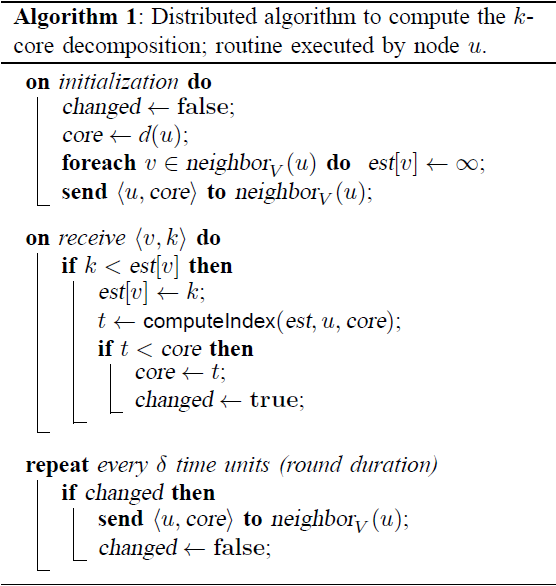
\includegraphics[width=90mm]{Algorithm1}
%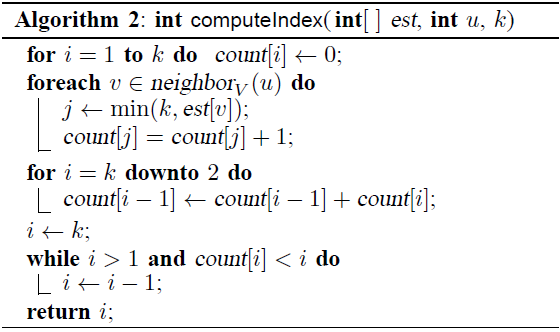
\includegraphics[width=90mm]{Algorithm2}
%\label{overflow}
%\end{figure}

Neste algoritmo cada vértice mantém um inteiro $core$, a estimação do seu \textit{coreness}, sendo iniciada com o seu grau. Um \textit{array} $est$ de estimativas das \textit{coreness} dos seus adjacentes, com todas as entradas iniciadas a infinito. %E uma flag $changed$ que é ativa se $core$ mudar.

\begin{algorithm}
\caption{k-Core Distribuído}
 \algorithmicrequire{Grafo não direcionado}

 \algorithmicensure{Tabela de vértices e a suas respetivas \textit{cores}}
\begin{enumerate}
	\item Na inicialização a sua $core$ deve ser iniciada com o grau do vértice e cada entrada de $est$ com infinito. Após, o vértice envia uma mensagem para todos os seus adjacentes com o seu $id$ e $core$.
	\item Ao receber uma mensagem cada vértice deve atualizar a sua estimativa da $coreness$ do remetente se esta for menor que a que tem atualmente
	\item Se atualizou a estimativa do adjacente deve computar uma nova possível estimativa e atualizar a sua $core$ com a nova estimativa caso esta seja menor que atual
	\item Se não mudou de core deve então tentar parar o algoritmo.
	\item Caso contrário volta e enviar uma mensagem para os seus vizinhos com o seu $id$ e a sua nova $core$
\end{enumerate}
\end{algorithm}

\begin{algorithm}
\caption{Computar uma nova estimativa}
 \algorithmicrequire{Vértice $v$ e $core$ atual do vértice}

 \algorithmicensure{Nova estimativa}
\begin{enumerate}
	\item Criar um \textit{array} $count$ de o tamanho $core+1$ com todas as entradas iniciadas a $0$.
	\item Para cada adjacente de $v$ calcular o mínimo entre a $core$ atual do vértice e a estimativa para o adjacente e incrementar a entrada de $count$ indexada por este mínimo.
	\item De $core$ a $a$ cada entrada de $count$ passa a ser a soma de si com a entrada anterior.
	\item Sendo que $i \gets core$, decrementar $i$ enquanto $i > 0$ e $count[i] < i$ e finalmente retornar este $i$.
\end{enumerate}
\end{algorithm}
Em modelos BSP uma vértice recebe todas as suas mensagens em simultâneo, logo é possível adiar o cálculo da nova estimativa para depois da atualização da estimativa de todos os adjacentes. 

Sabendo que a $core$ de um vértice só ajuda no cálculo de uma nova estimativa de um adjacente se esta for menor do que a estimativa atual $est$ no vértice basta enviar mensagens a estes adjacentes, reduzindo, assim, o número de mensagens durante o algoritmo.
%Distributed k-Core Decomposition

%http://arxiv.org/pdf/1103.5320v2.pdf

%http://arxiv.org/pdf/cs/0310049v1.pdf

%\bibliographystyle{plain}
%\bibliography{bibfiles}

